\chapter{Dataset}
\label{ch3}


\section{Weather Sequences}
Temporal sequence plots presented in Figure \ref{fig:sequence_temporal}.
\begin{figure}[p!]
	\centering
	\subfloat[Temperature (K)\label{fig:sequence_temporal_a}]{
		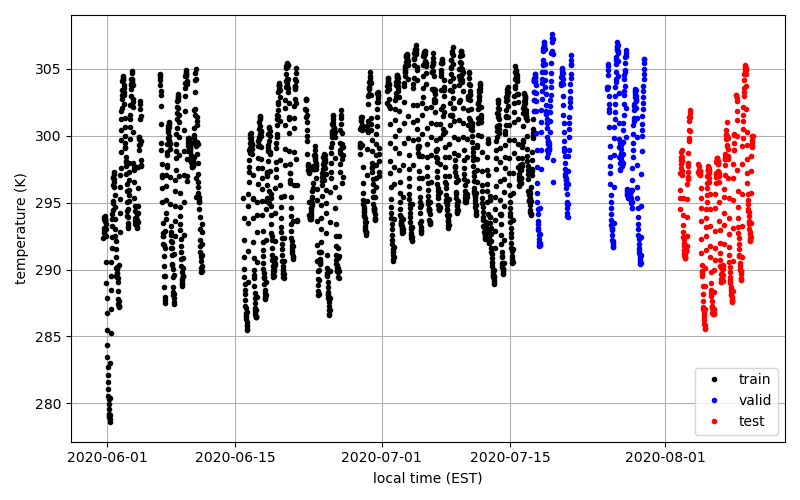
\includegraphics[width=0.49\textwidth]{temporal_sequence_temp.png}
	}
	\subfloat[Pressure (Pa)\label{fig:sequence_temporal_b}]{
		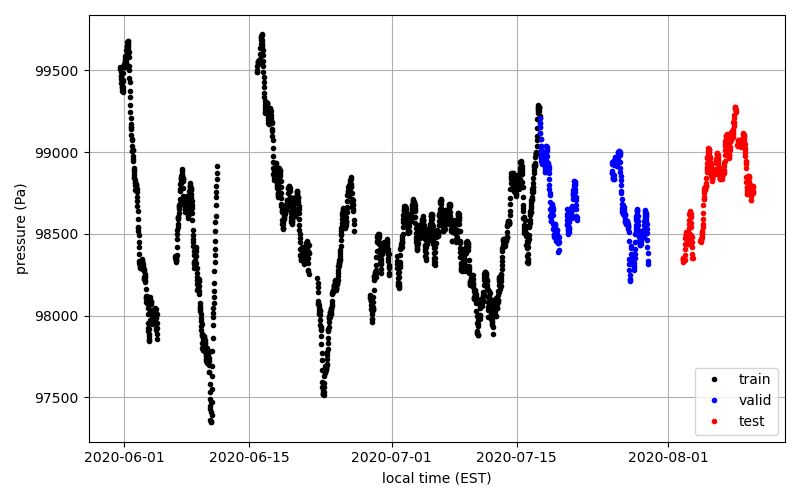
\includegraphics[width=0.49\textwidth]{temporal_sequence_press.png}
	}
	\hfill
	\subfloat[Relative Humidity (\%)\label{fig:sequence_temporal_c}]{
		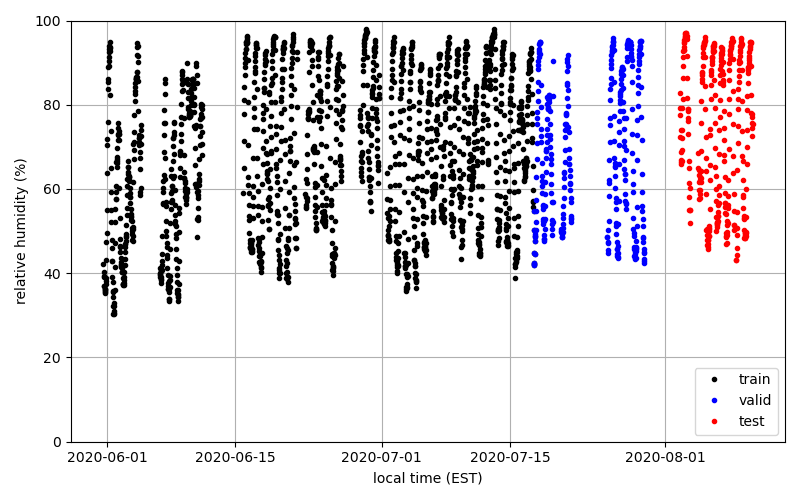
\includegraphics[width=0.49\textwidth]{temporal_sequence_rh.png}
	}
	\subfloat[Wind Speed (m/s)\label{fig:sequence_temporal_d}]{
		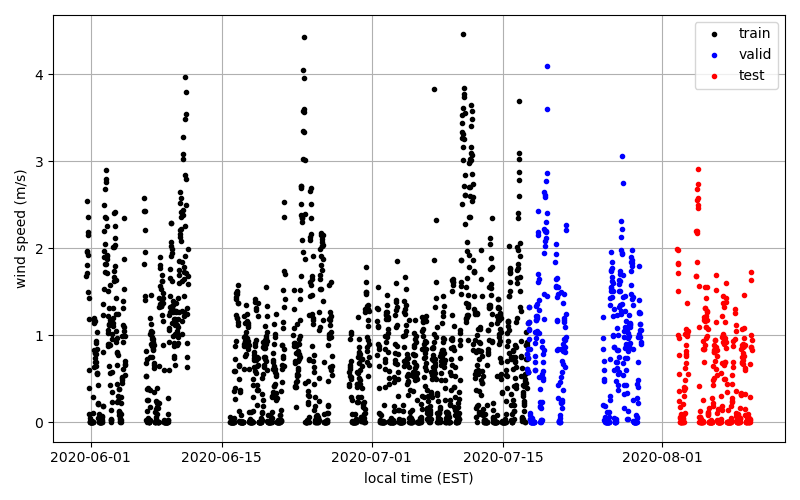
\includegraphics[width=0.49\textwidth]{temporal_sequence_wind_spd.png}
	}
	\hfill
	\subfloat[Solar Irradiance ($W/m^{2}$)\label{fig:sequence_temporal_e}]{
		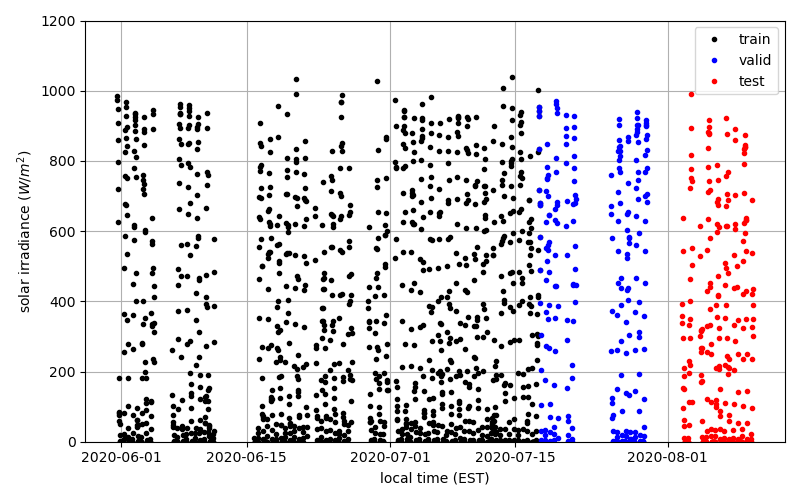
\includegraphics[width=0.49\textwidth]{temporal_sequence_solar_irr.png}
	}
	\subfloat[Turbulence $C_{n}^{2}$ ($m^{-2/3}$)\label{fig:sequence_temporal_f}]{
		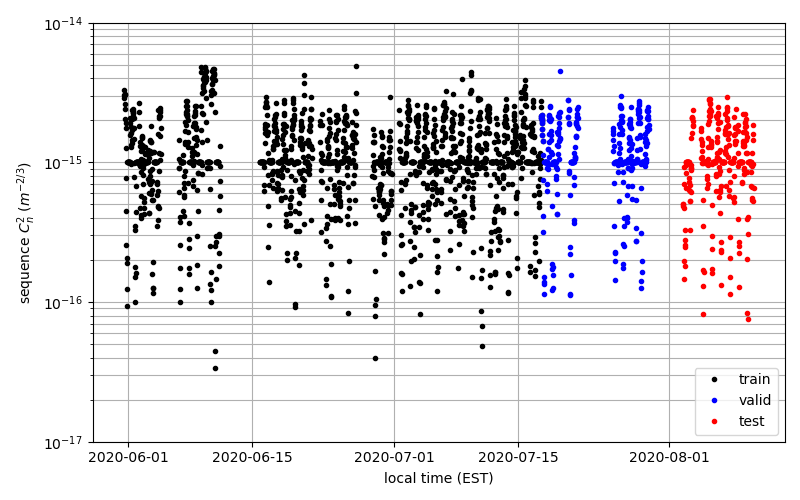
\includegraphics[width=0.49\textwidth]{temporal_sequence_cn2.png}
	}
	\hfill
	\caption{Sequence data as a function of time, parsed by train, validation, and test datasets drawn in black, blue, and red, respectively.}
	\label{fig:sequence_temporal}
\end{figure}

Histogram sequence plots presented in Figure \ref{fig:sequence_histograms}
\begin{figure}[p!]
	\centering
	\subfloat[Temperature (K)\label{fig:sequence_histograms_a}]{
		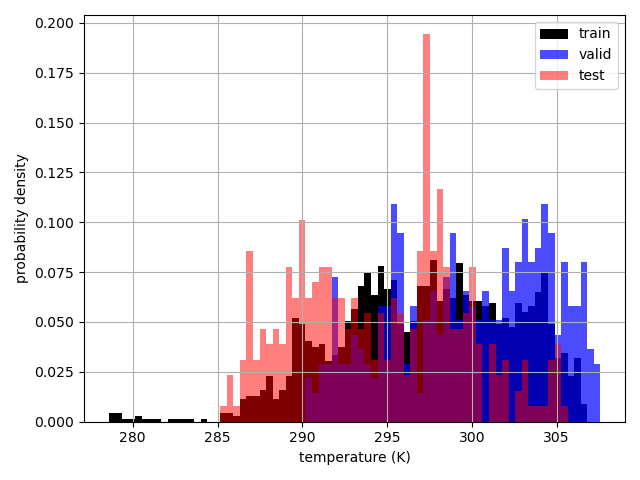
\includegraphics[width=0.49\textwidth]{hist_sequence_temp.png}
	}
	\subfloat[Pressure (Pa)\label{fig:sequence_histograms_b}]{
		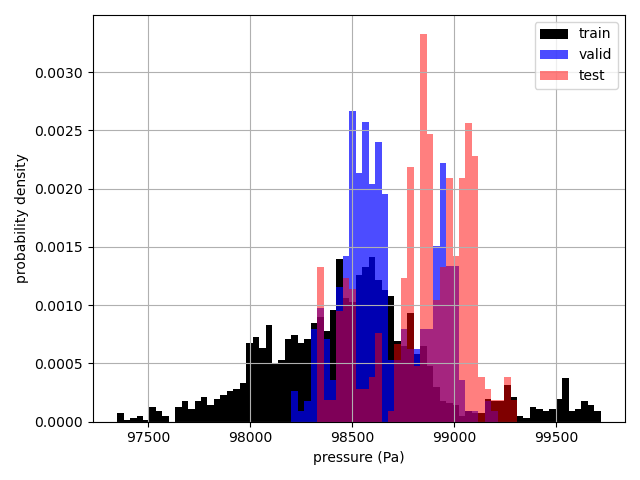
\includegraphics[width=0.49\textwidth]{hist_sequence_press.png}
	}
	\hfill
	\subfloat[Relative Humidity (\%)\label{fig:sequence_histograms_c}]{
	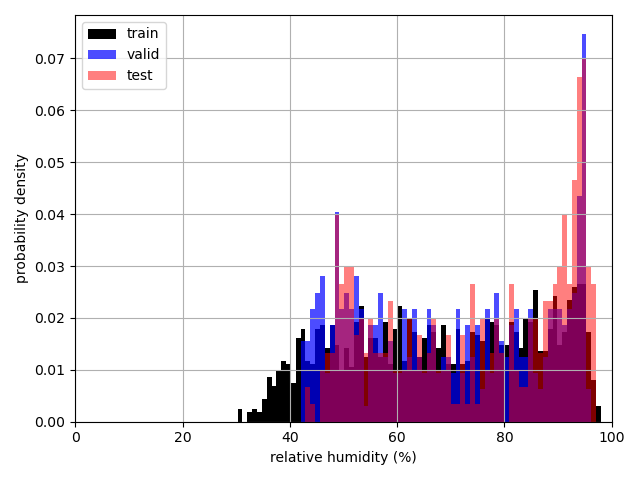
\includegraphics[width=0.49\textwidth]{hist_sequence_rh.png}
	}
	\subfloat[Wind Speed (m/s)\label{fig:sequence_histograms_d}]{
	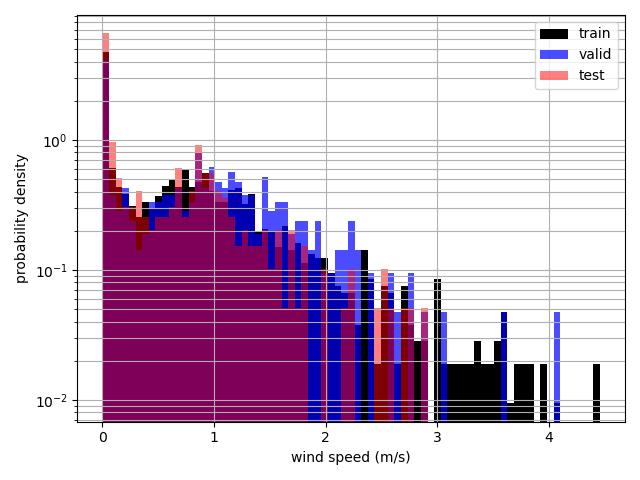
\includegraphics[width=0.49\textwidth]{hist_sequence_wind_spd.png}
	}
	\hfill
	\subfloat[Solar Irradiance\label{fig:sequence_histograms_e}]{
	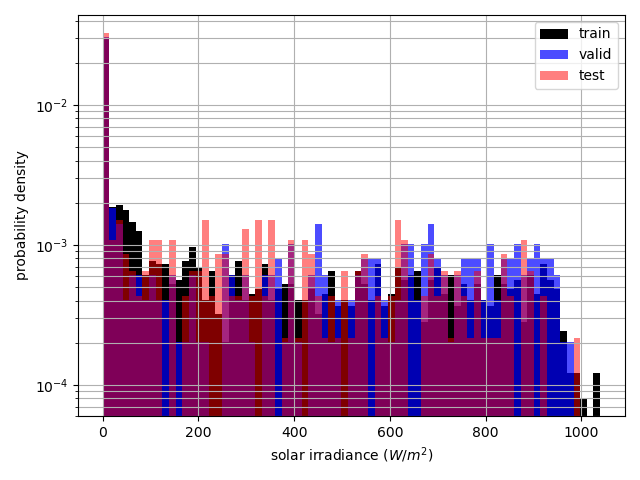
\includegraphics[width=0.49\textwidth]{hist_sequence_solar_irr.png}
	}
	\subfloat[$C_{n}^{2}$ ($m^{-2/3}$)\label{fig:sequence_histograms_f}]{
	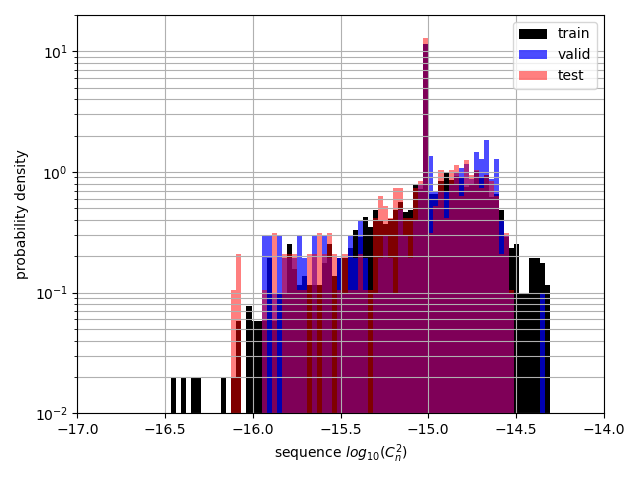
\includegraphics[width=0.49\textwidth]{hist_sequence_cn2.png}
	}
	\hfill
	\caption{Sequence data in normalized histograms, parsed by the train, validation, and test datasets drawn in black, blue, and red, respectively.}
	\label{fig:sequence_histograms}
\end{figure}

Forecast plots in Figure \ref{fig:forecast_sequence_histogram}
\begin{figure}[h!]
	\centering
	\subfloat[\label{fig:forecast_sequence_histogram_a}]{
		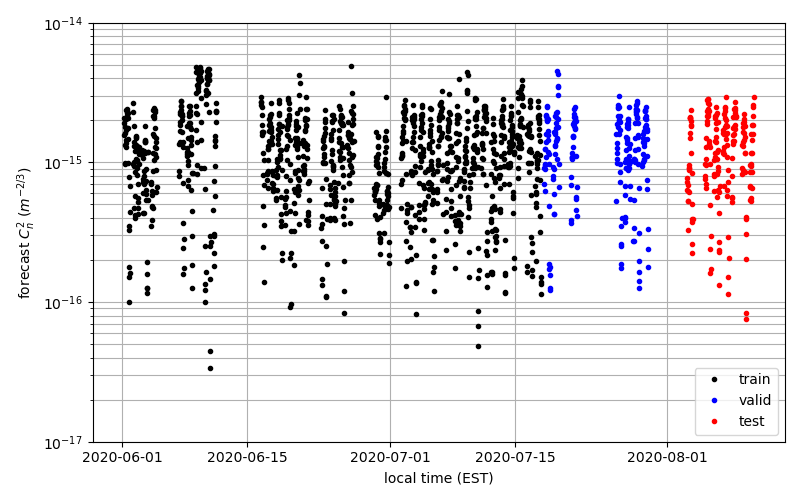
\includegraphics[width=0.543\textwidth]{temporal_forecast_cn2.png}
	}
	\subfloat[\label{fig:forecast_sequence_histogram_b}]{
		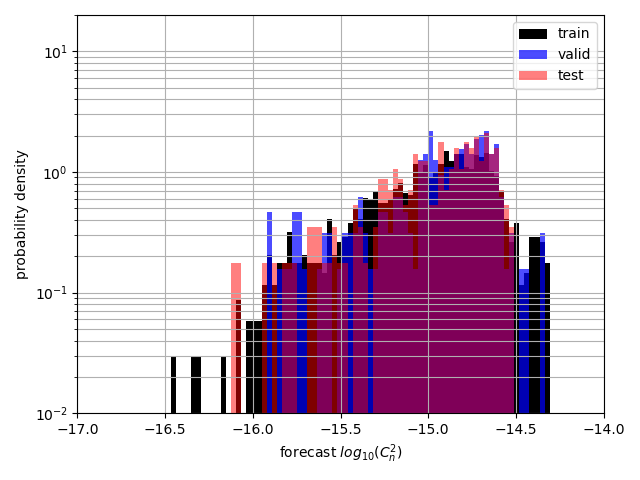
\includegraphics[width=0.447\textwidth]{hist_forecast_cn2.png}
	}
	\hfill
	\caption{Turbulence ($C_{n}^{2}$) forecasts as a function of time and as a normalized histogram. The train, validation, and test datasets are drawn in black, blue, and red, respectively.}
	\label{fig:forecast_sequence_histogram}
\end{figure}